\chapter{Funções}

Desde o final do século XIX, diversas áreas da matemática
estudam consistentemente \textit{\hyperlink{chapter.5}{conjuntos}},
\textit{\hyperlink{chapter.6}{relações}}, já apresentadas
nesse texto, e funções. Neste capítulo, debruçaremos nossa
atenção nas propriedades dessa terceira área.

Entende-se que uma função $f$ é um mapeamento entre um
domínio $X$ e um domínio $Y$, este que será conhecido como
contradomínio, posteriormente. Entretanto, para teóricos
de conjuntos, esses domínios são simplesmente considerados
conjuntos. Vimos que \textit{\hyperlink{chapter.2}{Lean}} é uma
linguagem baseada em Tipos. Dessa forma, estabelece-se uma
diferença clara entre o Domínio $X$, caracterizado pelos Tipos, e
o Conjunto $A$, que é do tipo (sub)conjunto de $X$. Em Lean:
\begin{lstlisting}
variable X : Type
variable A : set X
\end{lstlisting}

Entretanto a visão da função como mapeamento entre conjuntos
é comum entre os matemáticos e será considerada nesse texto,
fazendo as devidas comparações com a linguagem de referência,
o Lean.

\section{O Conceito de Função}
\label{concept}

Considere dois conjuntos quaisquer $X$ e $Y$ e um mapeamento $f$ do conjunto
$X$ para o conjunto $Y$. Se $f$ atribui um e apenas um valor para cada
elemento de $X$, dizemos que $f$ é uma função total e escrevemos $f: X \to Y$.
Chamamos $X$ de domínio de $f$, enquanto $Y$ é o contradomínio de $f$ e
$\forall x, (x \in X  \Rightarrow f(x) \in Y)$. Nesse sentido, $\forall x_1
\in X, \forall x_2 \in X, x_1 = x_2 \Rightarrow f(x_1) = f(x_2)$. Uma função
também pode ser parcial quando ela não é definida para alguns valores do
domínio. Escrevemos $f: X \nrightarrow Y $ para representar uma função parcial
definida em $A \subseteq X $, mas não definida no complementar de $A$. 

Um exemplo amplamente conhecido de funções parciais é $f: \mathbb{R}
\nrightarrow \mathbb{R}$, definida por $f(x) = \frac{1}{x}$, que é indefinida
em $x = 0$. Assim, na realidade, expressamos $f$ como $f : \mathbb{R}
\setminus \{0\} \to \mathbb{R}$. Alguns chamam $A$ de domínio de definição.
Como toda função parcial é total ao se restringir o domínio, trateremos nesse
texto das funções totais e a extensão das definições devido à parcialidade são
deixadas ao leitor.  

A maneira mais simples de se representar uma função é escrevê-la
explicitamente para cada elemento do domínio. Por exemplo, podemos escrever as
seguintes expressões:

\begin{itemize}
    \item Seja $f: \mathbb{N} \to \mathbb{N}$ definida por $f(n) = 2\cdot n +
    1$
    \item Seja $g : \mathbb{N} \to \mathbb{R}$ definida por $g(n) =
    \frac{n}{n+1}$
    \item Seja $h : \mathbb{R} \to \{0,1\}$ definida por
    $$\left \{ \begin{array}{c} h(x) = 1 ~if~x \in \mathbb{Q} \\
    h(x) = 0 ~ if ~ x \not \in \mathbb{Q} \\
    \end{array}
    \right. $$
 \end{itemize}

A questão que se levanta é: o que torna uma expressão explícita legítima?
Neste momento, deixaremos essa questão de lado e notaremos que a matemática é
confortável com diversos tipos de definições, como, por exemplo, a definição
de $h(x)$ no exemplo acima. Nesse mesmo exemplo, não fica claro em como
podemos definir algoritmicamente se um número real de entrada é um número
racional ou não. Porém, esse não é o objetivo do capítulo.

Note que a escolha das variáveis $x$ e $n$ são arbitrárias. Isto nos leva à
definição no Capítulo de \textit{\hyperlink{chapter.4}{FOL}} de variável
ligada (\textit{bound}), visto que se renomearmos $x$ com $y$, os valores
continuam os mesmos.

Lógicos frequentemente utilizam a notação $\lambda x ~e(x)$ para denotar a
função que mapeia $x$ para $e(x)$. Essa notação chama-se \textit{notação
lambda} e pode ser usada da seguinte forma: $f = \lambda x(x + 1)$, que
significa $f(x) = x + 1$. Essa notação é mais interessante para cientistas da
computação e lógicos do que propriamente para matemáticos. Em Lean, definimos
da seguinte forma:

\begin{lstlisting}
variables X Y : Type
variable f : X → Y

def square (n : ℕ) := n*n 

def double (n : ℕ) := 2*n

variable n: ℕ 

#check square n     -- square n : ℕ 

#reduce square 3    -- 9

#eval square 12120  -- #reduce 12120 return an error, because the 
                    -- calculation is by deep recursion

example (n : ℕ) : double 2 = square 2 :=
by rw [double, square]
\end{lstlisting}

Lembre-se que diferenciamos o tipo $X$ do tipo $set~X$ em Lean.

Outra forma comum de representar funções de forma didática é utilizando
gráficos, como podemos observar na Figura \ref{fig:functions-01-00}. Essa
representação tem uma limitação muito clara que é quando $X$ é um conjunto
infinito. Um conjunto é finito quando existe um número natural $n$ tal que
exista uma função $b$ bijetiva entre esse conjunto e o conjunto dos números
naturais menores ou iguais a $n$. 

A definição de função bijetiva pode ser encontrada na Definiçao \ref{def7},
enquanto maiores informações sobre os números naturais podem ser encontradas
no Capítulo de \textit{\hyperlink{chapter.8}{Indução dos Números Naturais}}.
Conjuntos encontram-se no \textit{\hyperlink{chapter.5}{Capítulo 5}}.

A partir de agora, vamos introduzir uma série de definições sobre a
terminologia que de funções, que acabamos de apresentar, e vamos extrair
proposições importantes a partir. 

\begin{figure}
    \centering      
    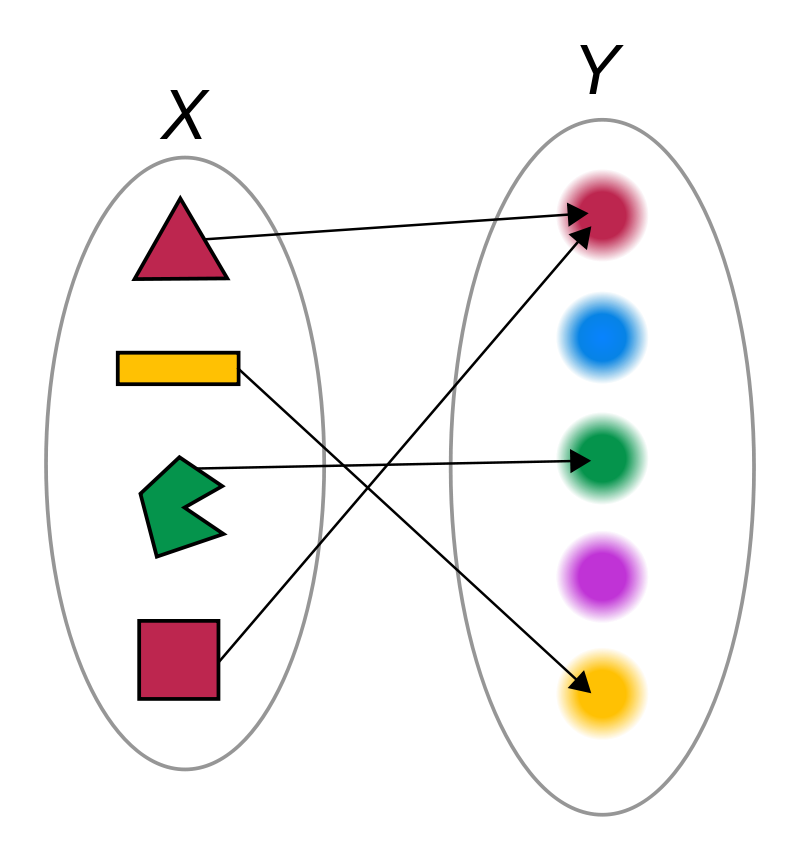
\includegraphics[width = 5cm]{figures/functions/fig-functions-01-00.png}
    \caption{Mapeamento entre o Domínio X e o Domínio Y, ambos não numéricos.}
    \label{fig:functions-01-00}
\end{figure}

\section{Primeiras Definições}

\theoremstyle{definition}
%\newtheorem{definition}{Definição}[section]

\theoremstyle{definition}
\newtheorem{example}{Exemplo}[section]

\theoremstyle{plain}
%\newtheorem{theorem}{Proposição}[section]

\theoremstyle{plain}
\newtheorem{corollary}{Corolário}[section]

\begin{definition}
    \label{def1}
    Seja um conjunto $A$. A função identidade de $A$ é a função
    $i_A : A \rightarrow A$ definida para todos os valores $x \in A$ tal que $i_A(x) = x$.
\end{definition}

\begin{definition}
    \label{def2}
    Sejam $f : X \rightarrow Y$ e $g : Y \rightarrow Z$ funções.
    Defina $k : X \rightarrow Z$ por $k(x) = g(f(x))$. A função $k$ é chamada de composição
    de $f$ e $g$ ou $f$ composta com $g$ e é escrita $g \circ f$. Desta forma, para cada elemento,
    primeiro  avaliamos $f(x) \in Y$ e depois avaliamos $g(f(x)) \in Z$.
\end{definition}

Podemos ver em Lean as definições de composição e de identidade. Note que estamos em um namespace
hidden para que não haja conflito de definições.

\begin{lstlisting}
namespace hidden
    variables {X Y Z : Type}

    def comp (f : Y → Z) (g : X → Y) : X → Z :=
    λx, f (g x)

    infixr  ` ∘ ` := comp

    #check @comp

    def id (x : X) : X := x

    #check @id

end hidden
\end{lstlisting}

\begin{definition}
    \label{def3}
    Considere $f,g : X \to Y$. Dizemos que essas funções são iguais,
    quando para todos os valores do domínio $X$, a correspondência no contradomínio $Y$ é a
    mesma. Em lógica simbólica, $\forall x (x \in X \to (f(x) = g(x)) \iff f = g $.
\end{definition}

Obseve que em termos de lógica formal de tipos, poderíamos reescrever como
$\forall x : X (f(x) = g(x)) \iff f = g$. Escrevemos essa equivalência entre lógica e funções
utilizando a extensionalidade das funções, muito semelhante à descrita no capítulo de
\textit{\hyperlink{chapter.5}{conjuntos}}. Por exemplo, se $f, g : \mathbb{R} \to \mathbb{R}$
definidas por $f(x) = x + 1$ e $g(x) = 1 + x$, então $f = g$, pois para cada valor de $x$, vale
a comutativade da soma.

Em lean, o comando \lstinline{funext} (de "function extensionality") prova a igualdade de funções.

\begin{lstlisting}
variables {X Y : Type}

example (f g : X → Y) (h : ∀ x, f x = g x) : f = g :=
    funext h
\end{lstlisting}

\begin{theorem}
    \label{prop1}
    Para todo $f: X \to Y$, $f \circ i_X = f$ e $i_Y \circ f = f$
\end{theorem}
\begin{proof}
    Seja $x$ um elemento qualquer de $X$. Então $(f \circ i_X)(x) = f(i_X(x)) = f(x)$
     e $(i_Y \circ f)(x) = i_Y(f(x)) = f(x)$, o que mostra a igualdade.
\end{proof}

No Lean, podemos mostrar essa proposição da seguinte forma. Para algumas funções, será necessário
escrevermos \lstinline{open function}.

\begin{lstlisting}
variables {X Y Z W : Type}

lemma left_id (f : X → Y) : id ∘ f = f := rfl

lemma right_id (f : X → Y) : f ∘ id = f := rfl

theorem comp.assoc (f : Z → W) (g : Y → Z) (h : X → Y) :
    (f ∘ g) ∘ h = f ∘ (g ∘ h) := rfl

\end{lstlisting}

\begin{definition}
    \label{def4}
    Suponha $f:X \to Y$ e $g : Y \to X$ satisfaz $g \circ f = i_X$. Assim,
    $g(f(x)) = i_X(x) = x$, para todos os elementos de $X$. Neste caso $g$ é dita inversa à esquerda
    de $f$ e $f$ é dita inversa à direita de $g$. Quando $g$ é inversa à direita e é inversa à esquerda
    de $f$, então $g$ é dita simplesmente inversa de $f$.
\end{definition}

\begin{example}
    \label{ex1}
    Defina $f,g : \mathbb{R} \to \mathbb{R}$ por $f(x) = x + 1$ e $g(x) = x - 1$. Então $g$
    é inversa à direita e à esquerda de $f$ e vice-versa.
\end{example}
\begin{example}
    \label{ex2}
    $\mathbb{R}^{+}$ denota os reais não negativos. Defina $f : \mathbb{R} \to \mathbb{R}^{+}$
    por $f(x) = x^2$ e defina $g : \mathbb{R}^2 \to \mathbb{R}$ por $g(x) = \sqrt{x}$. Então
    $f(g(x)) = (\sqrt{x})^2 = x$, para todo $x$ no domínio de $g$. Então $f$ é inversa à esquerda de $g$
    e $g$ inversa à direita de $f$. Por outro lado, $g(f(x)) = \sqrt{x^2} = |x|$. Logo $g$ não é inversa à
    esquerda de $f$ e $f$ não é inversa à direita de $g$.
\end{example}

\begin{theorem}
    \label{prop2}
    Suponha que $f : X \to Y $ tem inversa à esquerda, $h : Y \to X $ e uma inversa à direita, $k : Y \to X $.
    Então $h = k$.
\end{theorem}
\begin{proof}
    Seja $y \in Y$. $h(f(k(y))) = k(y)$, pois $h$ é uma inversa à esquerda de $f$.
    Por outro lado, $f(k(y)) = y$ e, portanto $h(f(k(y))) = h(y)$. Assim $k(y) = h(y) $ e as funções são iguais.
\end{proof}

Essa proposição pode também ser vista em Lean. Considerarei a prova utilizando táticas. O leitor pode estudar
aquela que sentir mais confortável. Note que neste exemplo, já foi necessário o \lstinline{namespace function},
visto que \lstinline{left_inverse} e \lstinline{right_inverse} já estão predefinidas.

\begin{lstlisting}
open function

variables {X Y Z: Type}

-- Term and Calc Mode
example (f: X → Y) (h: Y → X) (k: Y → X)
    (hf: left_inverse h f) (fk: right_inverse k f): h = k :=
    have H: ∀ ( x : Y ), h x = k x, from
        assume x,
        have h1: h (f (k x)) = k x , from calc
            h ( f (k x)) = k x: by apply hf,
        have h2: h (f (k x)) = h x, from calc
            h (f (k x)) = h x: by rw fk,
        show h x = k x, from eq.trans (eq.symm h2) h1,
    show h = k, from funext H

-- Tatics Mode
example (f: X → Y) (h: Y → X) (k: Y → X)
    (hf: left_inverse h f) (fk: right_inverse k f): h = k :=
    begin
        apply funext,
        assume x,
        have hf: h (f (k x)) = k x, by apply hf,
        rw ←hf,
        rw fk,
    end
\end{lstlisting}

\begin{theorem}
    \label{prop3}
    Seja $f: X \to Y$. Se a inversa de $f$ existe, então ela é única. Isto é, se $g_1, g_2: Y \to X$ são inversas
    de $f$, então $g_1 = g_2$
\end{theorem}
\begin{proof}
    Sabemos que $g_1$ é inversa à esquerda de $f$. Então,
    $$g_1(f(g_2(x))) = g_2(x), ~para~todos~os~valores~de~x.$$
    Também, $g_2$ é inversa de $f$. Então,
    $$g_1(f(g_2(x))) = g_1(x), ~para~todos~os~valores~de~x.$$ Logo $g_1 = g_2$.
\end{proof}

Quando a inversa de $f$ existe, então, podemos escrevê-la como $f^{-1}$. Dada a Definição \hyperlink{def4},
podemos afirmar que $(f^{-1})^{-1} = f$.

Observe que uma função pode possuir mais de uma função inversa à esquerda ou mais de uma função inversa
à direita. Ainda, quando uma função possui mais de uma função inversa à esquerda, ela não possui inversa
à direita. Se ela possuisse, ela seria igual a todas as funções inversas à esquerda pela Proposição \ref{prop2},
portanto elas seriam iguais, o que é uma contradição, por hipótese. O mesmo vale para inversas à direita.

\begin{theorem}
     \label{prop4}
     Seja $f: X \to Y $ e $g: Y \to Z$. Se $h: Y \to X$ e $k: Z \to Y$ são inversas à esqueda de $f$ e $g$,
     respectivamente, então $h \circ k$ é inversa à esquerda de $g \circ f$. O mesmo vale quando substituimos
     esquerda por direita na proposição.
\end{theorem}

\begin{proof}
 $(h \circ k)\circ(g \circ f)(x) = h(k(g(f(x)))) = h(f(x)) = x $. A demonstração quando substituimos a proposição
 de esquerda para direita é análoga e é deixada como exercício ao leitor.
\end{proof}

\begin{corollary}
    \label{cor1}
    Se $f: X \to Y$ e $g: Y \to Z$ possuem inversas, então $(f \circ g)^{-1}$ existe e
    $(f \circ g)^{-1} = f^{-1} \circ g^{-1}$.
\end{corollary}

\begin{proof}
    Segue diretamente da Proposição \ref{prop4} e Proposição \ref{prop2}.
\end{proof}

\section{Funções Injetiva, Sobrejetiva e Bijetiva}

\begin{definition}[Função Injetiva]
    \label{def5}
    Também conhecida como função injetora, é uma função em que elementos
    distintos do domínio são mapeados para elementos diferentes do
    contradomínio. Dessa forma, seja $f: X \to Y$. Se $\forall x_1 \in X,
    \forall x_2 \in X, x_1 \neq x_2 \Rightarrow f(x_1) \neq f(x_2) $, f é
    injetiva. A definição pode ser feita pela contrapositiva dessa afirmação,
    também. A definição pela contrapositiva será bastante utilizada nas
    demonstrações.
\end{definition}

\begin{definition}[Função Sobrejetiva]
    \label{def6}
    Também conhecida como função bijetora, é uma função em que todos os
    elementos do contradomínio estão na imagem da função. Dessa forma, seja
    $f: X \to Y$. Se $\forall y \in Y, \exists x \in X, f(x) = y$, f é
    sobrejetiva.
   \end{definition}

\begin{definition}[Função Bijetiva]
    \label{def7}
    Também conhecida como bijeção ou correspondência um a um, é uma função
    simultaneamente injetiva e sobrejetiva.
\end{definition}

Em Lean, essas definições são descritas no \lstinline{namespace function}.

\begin{example}
    Considere os conjuntos $X = \{1,2,3,4\}$, numéricos e $Y = \{John, Paul,
    George, Ringo\}$, não numérico.É possível construir uma função
    bijetiva entre $X$ e $Y$. Ainda mais, toda função sobrejetiva entre esses
    conjuntos é também injetiva e consequentemente bijetiva.
\end{example}

\begin{lstlisting}
variables {X Y: Type}

def injective (f : X → Y) : Prop :=
∀ x₁ x₂, f x₁ = f x₂ → x₁ = x₂

def surjective (f : X → Y) : Prop :=
∀ y, ∃ x, f x = y

def bijective (f : X → Y) := injective f ∧ surjective f
\end{lstlisting}

\begin{theorem}
    \label{prop5}
    Seja $f : X \to Y$.
    \renewcommand{\labelenumi}{\Roman{enumi}}
    \begin{enumerate}
        \item Se $f$ possui inversa à esquerda, $f$ é injetiva.
        \item Se $f$ possui inversa à direita, $f$ é sobrejetiva.
        \item Se $f$ possui inversa, $f$ é bijetiva.
    \end{enumerate}
\end{theorem}
\begin{proof}
    Para provar I), suponha que $f(x_1) = f(x_2)$ e que $g$ é inversa à
    esquerda de $f$. Assim $g(f(x_1)) = x_1$ e $g(f(x_2)) = x_2$. Portanto
    $x_1 = x_2$ e está provado. Para provar II), considere $h$ inversa à
    direita de $f$. Seja $y \in Y$ e $x = h(y)$. Então $f(x) = f(h(y)) = y$. A
    terceira sai diretemente das duas anteriores e da Proposição \ref{def2}. 
\end{proof}

\begin{lstlisting}
open function

variables {X Y : Type}

theorem inj_of_left_inverse {g : Y → X} {f : X → Y} :
left_inverse g f → injective f :=
    assume h, assume x₁ x₂, assume feq,
    calc x₁ = g (f x₁) : by rw h
        ... = g (f x₂) : by rw feq
        ... = x₂       : by rw h

theorem surj_of_right_inverse {g : Y → X} {f : X → Y} :
right_inverse g f → surjective f :=
    assume h, assume y,
    let  x : X := g y in
    have f x = y, from calc
        f x  = (f (g y))    : rfl
        ... = y            : by rw [h y],
    show ∃ x, f x = y, from exists.intro x this
\end{lstlisting}

\begin{theorem}
    \label{prop6}
    Seja $f: X \to Y$
    \renewcommand{\labelenumi}{\Roman{enumi}}
    \begin{enumerate}
        \item Se $X$ é não vazio e $f$ é injetiva, então $f$ possui inversa à
        esquerda.
        \item Se $f$ é sobrejetiva, então $f$ possui inversa à direita.
        \item Se $X$ é não vazio e $f$ é bijetiva, então $f$ possui inversa.
    \end{enumerate}
\end{theorem}

\begin{proof}
    Seja $\hat{x} \in X$. Defina uma função $g: Y \to X$ com $g(y) = x$, tal
    que $f(x) = y$, se $y$ pertence a imagem de $f$. Caso não pertença, defina
    $g(y) = \hat{x}$. Agora, assuma $x \in X$. Suponha que $g(f(x)) = x'$.
    Essa suposição é válida, pois $f(x) \in Y$. Pela definição de $g$, como
    $f(x)$ pertence a imagem de $f$, então $g(f(x)) = x'$, tal que $f(x') =
    f(x)$. Como $f$ é injetiva, temos que $x = x'$ e $g(f(x)) = x$ e g é
    inversa à esquerda de $f$. 

    Para a segunda afirmação, defina $h: Y \to X$, onde, para cada $y \in Y$,
    escolha um elemento $x \in X$, tal que $f(x) = y$. Note que a
    sobrejetividade garante a existência desse elemento, mas não garante a
    unicidade na escolha. Então $f(h(y)) = f(x) = y$, por definição de $h$.

    A fim de provar a terceira, basta as demonstrações das anteriores e da
    Proposição \ref{def2}. 
\end{proof}

Algumas observações sobre essa demonstração são importantes. Ao definir $g$ na
primeira parte, precisa-se decidir se $x \in X$ existe tal que $f(x) = y$.
Isso pode não ser algoritmicamente feito, logo $g$ poderia não ser computável.
Na construção de $h$, a prova requere que haja uma escolha de valor de $x$
entre os possíveis candidatos. Isto é uma versão do
\href{https://pt.wikipedia.org/wiki/Axioma_da_escolha#Enunciado}{\textit{axioma
da escolha}}. Este axioma foi muito debatido no século XX, mas hoje já é comum
para demonstrações. O paradoxo de Banach-Tarski é um argumento contra o
axioma. Um bom vídeo sobre o assunto pode ser encontrado nesse
\href{https://www.youtube.com/watch?v=s86-Z-CbaHA}{link}.

Utilizando conceitos e resultados da seção anterior, podemos provar a seguinte
proposição.

\begin{theorem}
    Seja $f: X \to Y$ e $g: Y \to Z$.
    \renewcommand{\labelenumi}{\Roman{enumi}}
    \begin{enumerate}
        \item Se $f$ e $g$ são injetivas, $g \circ f$ também será.
        \item Se $f$ e $g$ são sobrejetivas, $g \circ f$ também será.
    \end{enumerate}
\end{theorem}

\begin{proof}
    Basta aplicarmos a Proposição \ref{def4} e definirmos $h$ e $k$ como
    inversas à esquerda de $f$ e $g$ respectivamente. Logo $(h \circ k)$ é
    inversa à esquerda de  $(g \circ f)$ e, portanto, ela é injetiva.

    O mesmo vale para a segunda afirmação.
\end{proof}

\begin{lstlisting}
open function

namespace hidden
    variables {X Y Z : Type}

    theorem injective_comp {g : Y → Z} {f : X → Y}
    (Hg : injective g) (Hf : injective f) :
    injective (g ∘ f) :=
        assume x₁ x₂,
        assume : (g ∘ f) x₁ = (g ∘ f) x₂,
        have f x₁ = f x₂, from Hg this,
        show x₁ = x₂, from Hf this

    theorem surjective_comp {g : Y → Z} {f : X → Y}
        (hg : surjective g) (hf : surjective f) :
    surjective (g ∘ f) :=
    begin
        assume z,
        apply exists.elim (hg z),
        assume y (hy: g y = z),
        apply exists.elim (hf y),
        assume x (hx: f x = y),
        rw ←hx at hy,
        apply exists.intro x hy
    end

    theorem bijective_comp {g : Y → Z} {f : X → Y}
        (hg : bijective g) (hf : bijective f) :
        bijective (g ∘ f) :=
    have ginj : injective g, from hg.left,
    have gsurj : surjective g, from hg.right,
    have finj : injective f, from hf.left,
    have fsurj : surjective f, from hf.right,
    and.intro (injective_comp ginj finj)
                (surjective_comp gsurj fsurj)
end hidden
\end{lstlisting}

\begin{example}
    Considere $f: \mathbb{N} \to Y$, tal que $f(n) = 2n$. Podemos, ter:
    \begin{itemize}
        \item $Y = \mathbb{N}$. $f$ é injetiva, mas não é sobrejetiva.
        \item $Y = \mathbb{R}$. $f$ é injetiva, mas não é sobrejetiva.
        \item $Y = \{n \in \mathbb{N} | n~par\}$. $f$ é bijetiva.
    \end{itemize}
\end{example}

\section{Funções e Subconjuntos do Domínio}

Nós podemos querer saber o comportamento de uma função em algum subconjunto
$A$ de  $X$. Por exemplo, podemos dizer que $f$ é injetiva em $A$ se para todo
$x_1$ e $x_2$ em A, $f(x_1) = f(x_2) $ implicar $x_1 = x_2 $, por exemplo. A
diferença com relação à função parcial é que nesse caso, a função pode ser
definida em seu complementar. 

\begin{definition}
    \label{def8}
    Se $f$ é função de $X$ e $Y$, dizemos que $f[A]$ denota a imagem de $f$ em
    $A$, definido por $f[A] = \{y \in Y | ~\exists x \in A, y = f(x)\}$.
\end{definition}

\begin{theorem}
    \label{prop7}
    Seja $f: X \to Y $ e $A$ um subconjunto de $X$. Então, para todo $x$ em
    $A$, $f(x)$ está em $f[A]$.
\end{theorem}

\begin{proof}
    Por definição, $f(x) \in f[A] $ se, e somente se, existe $x'$ em $A$ tal
    que $f(x') = f(x)$. Isto vale para  $x' = x $.
\end{proof}

Em Lean, utilizando Táticas, esta prova pode ser apresentada da seguinte
forma: 

\begin{lstlisting}
import data.set 
open function

variables {X Y : Type}

example (f: X → Y) (A : set X) (a : X) (h: a ∈ A) : (f a) ∈ f '' A :=
begin 
    apply exists.intro a, 
    exact and.intro h (eq.refl (f a)),  
end   
\end{lstlisting}

\begin{theorem}
    \label{prop8}
    Seja $f: X \to Y$ e $g: Y \to Z$. Seja $A$ subconjunto de $X$. Então
    $$(g \circ f)[A] = g[f[A]]$$
\end{theorem}

\begin{proof}
    Seja $z \in (g \circ f)[A]$. Então, para algum $x \in A$, $z = (g \circ
    f)(x) = g(f(x))$. Pelo que acabamos de provar na Proposição \ref{prop8},
    $f(x) \in f[A]$. Novamente, pelo que acabamos de provar, $g(f(x)) \in
    g[f[A]] $.

    Alternativamente, seja $z \in g[f[A]]$. Então, existe $y$ em $f[A]$ tal
    que $f(y) = z$. Como $y \in f[A]$, existe $x \in A$, tal que $f(x) = y$.
    Então $(g \circ f)(x) = g(f(x)) = g(y) = z$, então $z \in (g \circ f)[A] $
\end{proof}

Uma prova de que a composição de funções sobrejetivas é sobrejetiva é a que
descrevemos cima, pois $f: X \to Y$ é sobrejetiva se, e somente se, $f[X] =
Y$.

Nós podemos ver $f$ como uma função de $A$, um subconjunto de $X$ a $Y$,
simplesmente ignorando o comportamento de $f$ nos elementos fora de $A$.

\begin{definition}
    \label{def9}
    Denotamos $f \upharpoonright A$ como restrição de $f$ para $A$. Isto é,
    dadas $f: X \to Y$ e $A \subseteq X$, $f \upharpoonright A : A \to Y$ é
    definida por $(f \upharpoonright A)(x) = x$, para todo $x$ em $A$.
\end{definition}

Agora, $f$ é injetiva em $A$ significa que a restrição de $f$ em $A$ é
injetiva.

\begin{definition}[Pré-imagem]
    \label{def10}
    Se $f: X \to Y$ e $B \subseteq Y$, então a pré-imagem de $B$ em $f$,
    denotado por $f^{-1}[B]$ é definida por $f^{-1}[B] = \{x \in X | f(x) \in
    B\}$. Ou seja, é o conjunto de elementos de $X$ que são mapeados em $B$.
\end{definition}

Note que essa definição faz sentido mesmo que $f$ não tenha inversa, visto que
dado $y \in B$ pode não haver $x \in X$ com a propriedade de $f(x) \in B$,
como podem ter vários. Se $f$ tem inversa ($f^{-1}$), então, para todo $y$ em
$B$, existe exatamente um elemento $x$ em $X$ com $f(x) \in B$. Neste caso,
dizemos que $f^{-1}[B]$ é a imagem de $B$ sobre $f^{-1}$ ou a pré-imagem de
$B$ sobre $f$.

Em Lean, a definição de Pré-imagem encontra-se na bilbioteca \textit{Mathlib}
e é definida da seguinte forma: 

\begin{lstlisting}
variables {X Y : Type}

def preimage (f : X → Y) (B : set Y) : set X := {x : X | f(x) ∈ B}

infix ` ⁻¹' `:80 := preimage
\end{lstlisting}


\begin{theorem}
    Seja $f: X \to Y$, $g: Y \to Z$ e $C \subseteq Z$. Então $$(g \circ
    f)^{-1}[C] = f^{-1}[g^{-1}[C]]$$.
\end{theorem}
\begin{proof}
    Para qualquer $y$, $y \in (g \circ f)^{-1}[C]$ se, e somente se, $g(f(y))$
    está em $C$. Isto acontece se, e somente se, $f(y) \in g^{-1}[C]$, o que
    acontece se, e somente se $y \in f^{-1}[g^{-1}[C]]$.
\end{proof}

Seguem algumas propriedades sobre imagens e pré-imagens. Aqui, $f$ denota uma
função arbitrária de $X$ em $Y$. $A, A_1, A_2, ...$ denotam subconjuntos
arbitrários de $X$, e $B, B_1, B_2,...$ denotam subconjuntos arbitrários de
$Y$.

\begin{enumerate}
    \item $A \subseteq f^{-1}[f[A]]$, e se $f$ é injetiva, $A = f^{-1}[f[A]]$.
    \item $f[f^{-1}[B]] \subseteq B$, e se $f$ é sobrejetiva, $B =
    f[f^{-1}[B]]$.
    \item Se $A_1 \subseteq A_2$, então $f[A_1] \subseteq f[A_2]$.
    \item Se $B_1 \subseteq B_2$, então $f^{-1}[B_1] \subseteq f^{-1}[B_2]$.
    \item $f[A_1 \cup A_2] = f[A_1] \cup f[A_2]$.
    \item $f^{-1}[B_1 \cup B_2] = f^{-1}[B_1] \cup f^{-1}[B_2]$.
    \item $f[A_1 \cap A_2] \subseteq f[A_1] \cap f[A_2]$ e, se $f$ é injetiva,
    $f[A_1 \cap A_2] = f[A_1] \cap f[A_2]$.
    \item $f^{-1}[B_1 \cap B_2] = f^{-1}[B_1] \cap f^{-1}[B_2]$.
    \item $f[A] \setminus f[B] \subseteq f[A\setminus B]$.
    \item $f^{-1}[A] \setminus f^{-1}[B] \subseteq f[A \setminus B]$.
    \item $f[A] \cap B = f[A \cap f^{-1}[B]]$.
    \item $f[A \cup f^{-1}[B]] \subset f[A] \cup B $.
    \item $A \cap f^{-1}[B] \subseteq f^{-1}[f[A] \cap B]$.
    \item $A \cup f^{-1}[B] \subseteq f^{-1}[f[A] \cup B]$.
\end{enumerate}

A partir de agora, vamos demonstrar algumas dessas proporições, ora com
descrições da demonstração e ora com provas em Lean. Tambémm sugerimos que
essas proposições sejam exercícios para a leitora ou o leitor.

\subsection{Demonstrações com linguagem natural}

\begin{theorem}[Item 7]
    \label{exerc1}
    Sejam $X$ e $Y$ conjuntos, $A_1, A_2 \in X$ e $f: X \to Y$.
\end{theorem}

\begin{proof}
    Se $y \in f[A_1 \cap A_2]$, temos que existe $x \in A_1 \cap A_2$, com
    $f(x) = y$. Nesse caso, $f(x) \in f[A_1]$, e $f(x) \in f[A_2]$, o que
    demonstra a primeira parte.

    Agora, suponha a injetividade de $f$. Suponha também que $y \in f[A_1]
    \cap f[A_2]$. Assim, existem $x_1 \in A_1$ e $x_2 \in A_2$, com as
    propriedades de $f(x_1) = y = f(x_2)$. Como a função é injetiva, $f(x_1) =
    f(x_2) \Rightarrow x_1 = x_2$. Assim $x_1 \in A_2$, que implica $x_1 \in
    A_1 \cap A_2$. Logo, $y \in f[A_1 \cap A_2]$.
\end{proof}

\begin{theorem}[Item 11]
    \label{exerc2}
    Sejam $X$ e $Y$ conjuntos, $f: X \to Y, A \subseteq X$ e $B \subseteq Y$.
    Então, $f[A] \cap B = f[A \cap f^{-1}[B]]$
\end{theorem}

\begin{proof}
    Suponha, inicialmente, que $y \in f[A] \cap B$. Então $y \in B$ e para
    algum $x \in A$, $f(x) = y$. Nesse sentido, $x \in f^{-1}[B]$. Assim, $x
    \in A \cap f^{-1}[B]$ e, portanto, $y \in f[A \cap f^{-1}[B]]$.

    Alternativamente, se $y \in f[A \cap f^{-1}[B]]$, existe $x \in A \cap
    f^{-1}[B]$, com $f(x) = y$. Daqui, concluímos que $y = f(x) \in f[A]$ e $y
    \in B$, pela definição de pré-imagem. Então $y \in f[A] \cap B$, como
    queríamos provar.
\end{proof}

\begin{theorem}[Item 13]
\end{theorem}

\begin{proof}
    Suponha que $x \in A \and f^{-1}[B]$. Desta maneire, $x \in A$ e $x \in
    f^{-1}[B]$, que implica que existe $y \in B$, tal que $f(x) = y$. Nesse
    sentido, $y \in B$ e $y \in f[A]$, que implica $y \in f[A] \and B$. Como
    $f(x) = y $, então $x \in f^{-1}[f[A]\and B]$. 

\end{proof}

\subsection{Demontrações em Lean}

Nós podemos utilizar variáveis limitadas para falar sobre o comportamento de
funções em conjuntos particulares.

\begin{lstlisting}
import data.set -- inclui o símbolo de subconjunto da imagem ''
open set function

variables {X Y : Type}
variables (A  : set X) (B : set Y)

def maps_to (f : X → Y) (A : set X) (B : set Y) :=
    ∀ x ∈ A, f x ∈ B

def inj_on (f : X → Y) (A : set X) :=
    ∀ (x₁ ∈ A) (x₂ ∈ A), f x₁ = f x₂ → x₁ = x₂

def surj_on (f : X → Y) (A : set X) (B : set Y) :=
    B ⊆ f '' A

\end{lstlisting}

A definição de \lstinline{maps_on} é a ideia de que a imagem de um subconjunto
do domínio $X$ está totamente inclusa em um subconjunto específico do
contradomínio. As definições de \lstinline{inj_on} e \lstinline{surj_on} são
as definições usuais.

\begin{theorem}[Item 1]
\end{theorem}

\begin{lstlisting}
import data.set 
open function
open set 

variables {X Y : Type}

theorem item1.a (f : X → Y) (A : set X) : A ⊆  f ⁻¹' (f '' A) := 
assume a h, 
have h1: a ∈ A ∧ f a = f a, from and.intro h (eq.refl (f a)),
have h2: (f a) ∈ f '' A, from exists.intro a h1,   
show a ∈ f ⁻¹' (f '' A), from h2

theorem item1.b (f : X → Y) (A : set X) (h: injective f): 
        A =  f ⁻¹' (f '' A) :=
eq_of_subset_of_subset
(item1.a f A)
(assume x h1, 
have h2: f x ∈ f '' A, from h1,
have h3: ∃ (a : X), a ∈ A ∧ f a = f x, from h1,
show x ∈ A, from exists.elim h3
    (assume (y : X) (h4: y ∈ A ∧ f y = f x),
    have h5: y = x, from h h4.right,
    show x ∈ A, from eq.subst h5 h4.left)
)
\end{lstlisting}

\begin{theorem}[Item 3]
\end{theorem}

\begin{lstlisting}
import data.set
open set function

variables {X Y : Type}
variables (A B A₁ A₂ : set X)

theorem item3 (f: X → Y) : A₁ ⊆ A₂ → f '' A₁ ⊆ f '' A₂ :=
    assume h : A₁ ⊆ A₂,
    assume y,
    assume h₁ : y ∈ f '' A₁,
    have h₂ : ∃ x, x ∈ A₁ ∧ f(x) = y, from h₁,
    show y ∈ f '' A₂, from exists.elim h₂
        (assume (x' : X) (ha: x' ∈ A₁ ∧ f(x') = y ),
        have h₃ : x' ∈ A₂ ∧ f(x') = y, from and.intro (h ha.left)  ha.right,
        show y ∈ f '' A₂, from exists.intro x' h₃)    
\end{lstlisting}

\begin{theorem}[Item 9]
\end{theorem}

Observe que para o item 9, trataremos $X$ e $Y$ como conjuntos iguais. Caso
não sejam, $f[B]$ pode nem estar definida.

\begin{lstlisting}
import data.set
open set function

variables {X Y : Type}
variables (A B A₁ A₂ : set X)

theorem item9 (f: X → X) : f '' A \ f '' B ⊆ f '' (A \ B) :=
begin
    intros y h,
    have h₁ : y ∈ f '' A, from mem_of_mem_diff h,
    have h₂ : ¬ (y ∈ f '' B), from not_mem_of_mem_diff h,
    apply exists.elim h₁,
    intros x h₃,
    apply exists.intro x,
    apply and.intro,
    apply mem_diff_of_mem,
        exact h₃.left,
        assume h₄ : x ∈ B,
        exact false.elim (h₂ (exists.intro x (and.intro h₄ h₃.right))),
        exact h₃.right
end

#check @mem_of_mem_diff
#check @not_mem_of_mem_diff
#check @mem_diff_of_mem

\end{lstlisting}

As funções \lstinline{mem_of_mem_diff, not_mem_of_mem_diff} e
\lstinline{mem_diff_of_mem} tem o objetivo de lidar com a diferença e sua
relação com a interseção. Note que usar táticas auxilia o passo a passo, porém
dificulta o posterior entendimento. Por isso, é recomendável, nesses exemplos,
utilizar alguma ferramenta para Lean. Essas funções e outras já apresentadas,
encontram-se na biblioteca do Lean e grande parte delas está disponível quando
você abre o namespace \lstinline{function}.

\begin{lstlisting}
open function 

#check @comp 
#check @has_left_inverse
-- A right_inverse tem duas definicoes para Lean. Apenas uma
-- esta no namespace function. Por isso e importante especificar. 
#check @function.right_inverse    
\end{lstlisting}

\subsection{Definindo a inversa Classicamente}

Para definir funções inversas, é necessário que utilizemos o racionínio
clássico. 

\begin{lstlisting}
open classical 

#check @axiom_of_choice
#check @some_spec

variables A B : Type
variable P : A → Prop   
variable R : A → B → Prop

example : (∀ x, ∃ y, R x y) → ∃ f : A → B, ∀ x, R x (f x) :=
axiom_of_choice

example (h : ∃ x, P x) : P (some h) :=
some_spec h    
\end{lstlisting}

O axioma da escolha fala que se para todo \lstinline{x : X}, existe
\lstinline{y: Y} com \lstinline{R x y}, então existe uma função \lstinline{f: X → Y} que para todo \lstinline{x}, escolhe-se \lstinline{y}. Em Lean, é
utilizada a função \lstinline{some} para mostrar este axioma, através da
construção clássica. Podemos, portanto, definir a inversa como: 

\begin{lstlisting}
open classical function
local attribute [instance] prop_decidable

variables {X Y : Type}

noncomputable def inverse (f : X → Y) (default : X) : Y → X :=
λ y, if h : ∃ x, f x = y then some h else default   
\end{lstlisting}

Observe que a definição é não computacional, visto que como já argumentamos,
para uma determinada função, essa hipótese \lstinline{h} pode não ser possível
de validar algoritmicamente e, se a hipótese for válida, pode não ser possível
encontrar um valor de \lstinline{x} adequado, também algoritmicamente. Também
observe que essa inversa é definida assumindo \lstinline{y}, logo ela é
definida para todo valor que ele assume e retorna algum valor qye cumpre essa
propriedade \lstinline{f x = y}, quando a hipótese é válida, ou um valor
padrão dado inicialmente, caso não exista. O comando \lstinline{local attribute} 
fala para a instância que a regra \lstinline{prop_decidable} vai
ser utilizada no arquivo que se segue. Nesse caso, importamos os axiomas
clássicos e tornamos disponível a instância genérica da decição.   

Podemos, então, demonstrar os seguintes teoremas. 

\begin{lstlisting}
open classical function
local attribute [instance] prop_decidable

variables {X Y : Type}

noncomputable def inverse (f : X → Y) (default : X) : Y → X :=
λ y, if h : ∃ x, f x = y then some h else default

theorem inverse_of_exists (f : X → Y) (default : X) (y : Y)
    (h : ∃ x, f x = y) : f (inverse f default y) = y :=
    have h₁ : inverse f default y = some h, from dif_pos h,
    have h₂ : f (some h) = y, from some_spec h,
eq.subst (eq.symm h₁) h₂

#check @dite
#check @dif_pos 

-- Using Term Mode 
theorem is_left_inverse_of_injective (f : X → Y) (default : X)
    (injf : injective f) : left_inverse (inverse f default) f :=
let finv := (inverse f default) in
    assume x,
    have h1 : ∃ x', f x' = f x, from exists.intro x rfl,
    have h2 : f (finv (f x)) = f x, 
        from inverse_of_exists f default (f x) h1,
    show finv (f x) = x, from injf h2

-- Using Tatic Mode 
theorem is_left_inverse_of_injective2 (f : X → Y) (default : X)
    (injf : injective f) : left_inverse (inverse f default) f :=
begin 
    intro x,
    apply injf, 
    apply inverse_of_exists,
    apply exists.intro x,
    exact eq.refl (f x), 
end
\end{lstlisting}

Observado o significado de \lstinline{dite}, que expressa a validade de um
\lstinline{α : Sort}, independente de \lstinline{c: Prop} e o significado de
\lstinline{dif_pos}, que expressa a igualdade entre uma expressão do formato
\lstinline{dite} e outra do mesmo \lstinline{Sort}, podemos entender o
siginificado dessa prova. A versão em Táticas foi inserida como instrução de
aplicação em comparação como o modo em termos. 

\section{Lógica de Segunda ou Mais Alta Ordem}

Até agora, formalmente, definimos lógica de primeira ordem, onde iniciamoscom um estoque 
fixo de símbolos de funções e relações, nos últimos tópicos que  consideramos, ocorre a motivação 
de extender a linguagem para funções e relações. Por exemplo, ao afirmar que $f: X \to Y$ possui 
inversa a esquerda pode ser dito como: $$\exists g, \forall x, g(f(x)) = x.$$
Outro exemplo é o seguinte teorema, descrito em linguagem lógica 
$$\forall x_1, x_2, (f(x_1) = f(x_2) \to x_1 = x_2) \to \exists g, \forall x, g(f(x)) = x.$$
Isto é, se $f: X \to Y$ é injetiva, então existe inversa à sua esquerda.

Nesse sentido, existe uma quantificação sobre as funções e relações, o que se distancia do que a lógica 
de primeira ordem cobre. Como forma de resolver esse impasse, podemos desenvolver uma teoria na linguagem 
de lógica de primeira ordem no qual o universo contém funções e relações como objetos ou extender essa linguagem
para envolver novos tipos de quantificadores e variáveis, que é o caso descrito nessa sessão. Isto é o que Lógica
de Ordem mais Alta faz. 

Alonzo Church (1903 - 1995) foi um matemático e lógico estadunidense, conhecido pelo cálculo lambda, formulou a ideia
de ordens mais altas na lógica. Isso é algumas vezes descrito como Teoria Simples dos Tipos ou Teoria dos Tipos de 
Chunch's. Sejam $X, Y, Z,...$ tipos básicos e $Prop$ um tipo especial das proposições. Temos, então:
\begin{itemize}
    \item Se $X$ e $Y$ são tipos, então $U \times V$ também será.Isto denota que o par ordenado $(x,y)$, com $x \in X$ 
    e $y \in Y$ é tipado. 
    \item Se $X$ e $Y$ são tipos, então $U \to V$ também será.
\end{itemize}

Para formar expressões, a teoria de Church aficiona os seguintes caminhos: 
\begin{enumerate}
    \item Se $x$ é do tipo $X$ e $y$ é do tipo $Y$, $(x,y)$ é do tipo $X \times Y$. 
    \item Se $z$ é do tipo $X \times Y$, então $(p)_1$ é do tipo $X$ e $(p)_2$ é do tipo $Y$, que denotam o primeiro e 
    segundo elemento do par $z$, respectivamente. 
    \item Se $x$ é uma variável do tipo $X$ e $y$ é uma expressão do tipo $Y$, então $\lambda x y$ é do tipo $X \to Y$. 
    Para lembrar o significado dessa expressão, voltar em \ref{concept}.
    \item Se $f$ é do tipo $X \to Y$ e $x$ é do tipo $X$, $f(x)$ é do tipo $Y$. 
\end{enumerate}

Além desses meios, a teoria simples dos tipos possui conetivos booleanos, quantificadores e a igualdade, oriunda da lógica
de primeira ordem, para construir proposições. 

A fução $f(x,y)$ que toma elementos de $X$ e $Y$ para o tipo $Z$ é vista como um objeto do tipo $X \times Y \to Z$. Note que,
nesse sentido, uma relação binária $R(x,y)$ definida em $X$ e $Y$ é vista como um objeto $X \times Y \to Prop$. O que torma essa 
lógica ser de ordem mais alta é que podemos iterar o tipo função indefinidamente. Por exemplo, se $\mathbb{N}$ é o tipo dos números
naturais, $\mathbb{N} \to \mathbb{N}$ denota o tipo das funções dos números naturais aos números naturais, e $(\mathbb{N} \to \mathbb{N}) \to \mathbb{N}$ 
denota o tipo de funções $F(f)$ que tomam uma função como argumento e retornam um número natural. Vamos ver em Lean:

\begin{lstlisting}
open nat 

#check ℕ                -- ℕ : Type
#check ℕ → ℕ            -- ℕ → ℕ : Type
#check (ℕ → ℕ) → ℕ      -- (ℕ → ℕ) → ℕ : Type 

variable F: (ℕ → ℕ) → ℕ 
variable f: ℕ → ℕ
variable n: ℕ 

#check f n              -- f n : ℕ 
#check F f              -- F f : ℕ 
#check F n              -- error
\end{lstlisting}

A variavél $F$ espera uma função, por isso retorna erro no último \lstinline{#check}. Se retirarmos o parênteses, Lean entenderá que 
\lstinline{F : ℕ → (ℕ → ℕ)}. 

As especificações de síntaxe e regras da lógica de ordem mais alta são descritas mais cuidadosamente em livros-texto mais avançados. 
Para considerar os tipos de funções e relações, basta o conhecimento de lógica de segunda ordem. É importante ter em mente que já lidamos 
desde os primeiros capítulos com os tipos e lógica de segunda ordem, em Lean, que é um sistema de lógica ainda mais elaborado e expressivo. 

\subsection{Definindo a inversa Classicamente}

Para definir funções inversas, é necessário que utilizemos o racionínio clássico. 

\begin{lstlisting}
open classical 

#check @axiom_of_choice
#check @some_spec

variables A B : Type
variable P : A → Prop   
variable R : A → B → Prop

example : (∀ x, ∃ y, R x y) → ∃ f : A → B, ∀ x, R x (f x) :=
axiom_of_choice

example (h : ∃ x, P x) : P (some h) :=
some_spec h    
\end{lstlisting}

O axioma da escolha fala que se para todo \lstinline{x : X}, existe \lstinline{y: Y} com 
\lstinline{R x y}, então existe uma função \lstinline{f: X → Y} que para todo \lstinline{x},
escolhe-se \lstinline{y}. Em Lean, é utilizada a função \lstinline{some} para mostrar este a 
axioma, através da construção clássica. Podemos, portanto, definir a inversa como: 

\begin{lstlisting}
open classical function
local attribute [instance] prop_decidable

variables {X Y : Type}

noncomputable def inverse (f : X → Y) (default : X) : Y → X :=
λ y, if h : ∃ x, f x = y then some h else default   
\end{lstlisting}

Observe que a definição é não computacional, visto que como já argumentamos, para uma determinada função, essa 
hipótese \lstinline{h} pode não ser possível de validar algoritmicamente e, se a hipótese for válida, pode não 
ser possível encontrar um valor de \lstinline{x} adequado, também algoritmicamente. Também observe que essa inversa é 
definida assumindo \lstinline{y}, logo ela é definida para todo valor que ele assume e retorna algum valor qye cumpre 
essa propriedade \lstinline{f x = y}, quando a hipótese é válida, ou um valor padrão dado inicialmente, caso não exista. 
O comando \lstinline{local attribute} fala para a instância que a regra \lstinline{prop_decidable} vai ser utilizada no 
arquivo que se segue. Nesse caso, importamos os axiomas clássicos e tornamos disponível a instância genérica da decição.   

Podemos, então, demonstrar os seguintes teoremas. 

\begin{lstlisting}
open classical function
local attribute [instance] prop_decidable

variables {X Y : Type}

noncomputable def inverse (f : X → Y) (default : X) : Y → X :=
λ y, if h : ∃ x, f x = y then some h else default

theorem inverse_of_exists (f : X → Y) (default : X) (y : Y)
    (h : ∃ x, f x = y) : f (inverse f default y) = y :=
    have h₁ : inverse f default y = some h, from dif_pos h,
    have h₂ : f (some h) = y, from some_spec h,
eq.subst (eq.symm h₁) h₂

#check @dite
#check @dif_pos 

-- Using Term Mode 
theorem is_left_inverse_of_injective (f : X → Y) (default : X)
    (injf : injective f) : left_inverse (inverse f default) f :=
let finv := (inverse f default) in
    assume x,
    have h1 : ∃ x', f x' = f x, from exists.intro x rfl,
    have h2 : f (finv (f x)) = f x, 
        from inverse_of_exists f default (f x) h1,
    show finv (f x) = x, from injf h2

-- Using Tatic Mode 
theorem is_left_inverse_of_injective2 (f : X → Y) (default : X)
    (injf : injective f) : left_inverse (inverse f default) f :=
begin 
    intro x,
    apply injf, 
    apply inverse_of_exists,
    apply exists.intro x,
    exact eq.refl (f x), 
end
\end{lstlisting}

Observado o significado de \lstinline{dite}, que expressa a validade de um 
\lstinline{α : Sort}, independente de \lstinline{c: Prop} e o significado 
de \lstinline{dif_pos}, que expressa a igualdade entre uma expressão do formato 
\lstinline{dite} e outra do mesmo \lstinline{Sort}, podemos entender o siginificado
dessa prova. A versão em Táticas foi inserida como instrução de aplicação em comparação
como o modo em termos. 

\section{Funções e Relações}

Podemos ver que nem toda relação é uma função. Uma relação binária $R(x,y)$ em $A$ e $B$ 
é um \textit{funcional} se para todo $x$ em $A$, existe um valor único $y$ em $B$ tal que 
$R(x,y)$. Se $R$ é uma relação funcional, podemos definir $f_R: X \to B$ fazendo com que 
$f_R(x)$ seja igual ao valor de $y$ único em $B$ em que a relação seja verdadeira. A 
contrapartida é verdadeira, basta definir, para $f: X \to B$, $R_f(x,y)$, uma relação funcional. 
Essa relação é conhecida como o \textit{grafo de f}. 

Podemos extrair dessa ideia que existe uma dualidade entre uma relação funcional $R$ e uma 
função $f$. Inclusive, muitas vezes, as definições são intercambiáveis. Em fundamentos tipo-teóricos, 
como a que vemos em Lean, relações são frequentemente definidas como uma classe de funções, enquanto 
para fundamentos teóricos em conjuntos definem função como uma relação funcional. 

Podemos considerar funções $f(x,y)$ ou $g(x,y,z)$ que tomam múltiplos argumentos. Por exemplo, 
$f(x,y) = x + y$. Em lean, podemos exemplificar da seguinte forma: 

\begin{lstlisting}
variables X Y : Type 
variable f: X → X → X → Y 
variables x₁ x₂ x₃  : X

#check f x₁ x₂ x₃ -- tipo Y

def g (x y : ℤ): ℤ := x + y

example : g 1 1 = 2 := 
calc 
g 1 1 = 1 + 1 : by rw g 
    ... = 2 :  rfl
\end{lstlisting}

O número de argumentos de uma função é chamado de \textit{aridade}, que em inglês é \textit{arity}. 
No exemplo acima $f$ tem aridade $3$, enquanto $g$ tem aridade $2$.
Podemos pensar uma função com múltiplos argumentos como uma função unária definida em um produto cartesiano. 
Nesse sentido, quando estamos nos tratando de teoria dos tipos, é conveniente pensar que $f$ é uma função de $X$
que retorna uma função $X \to X \to Y$. Desta maneira, $f(x_1, x_2, x_3)$ abrevia $((f(x_1))(x_2))(x_3)$.

\begin{example}[Teorema de Cantor]
    \label{cantor}
    Seja $f$ uma função que mapeia elementos do conjunto $A$ para o seu conjunto das partes $P(A)$. Então $f: A \to P(A)$ 
    não é sobrejetiva. 
    Esse teorema é um teorema fundamental sobre conjuntos que foi apresentada nesse capítulo devido às definições importantes
    de funções. A referência é no capítulo sobre \hyperlink{chapter.5}{Conjuntos}. A demonstração se dá por contradição e é realizada
    no Lean com o auxílio do \lstinline{namespace classical}. 

    \begin{lstlisting}
    import data.set

    variables X Y: Type 
    
    def surjective {X: Type} {Y: Type} (f : X → Y) : Prop := ∀ y, ∃ x, f x = y
    
    theorem Cantor : ∀ (A: set X), ¬ ∃ (f: A → set A),  surjective f :=
    
        begin
            intro A,
            intro h,
            -- Utiliza a regra eliminação existe.
            cases h with f h1,
            -- Como f é sobrejetiva e esse é um subconjunto de A            
            have h2: ∃ x, f x = {t : A | ¬ (t ∈ f t)},  
                from h1 {t : A | ¬ (t ∈ f t)},
            -- Eliminação do existe, novamente. 
            cases h2 with x h3,
            -- classical.em A := A ∪ ¬A é uma tautologia. 
            apply or.elim (classical.em 
                          (x ∈ {t : A | ¬ (t ∈ f t)})),
                intro h4,
            -- Usa a proriedade do conjunto
                    have h5: ¬ (x ∈ f x), from h4,
                    rw (eq.symm h3) at h4, 
                    apply h5 h4,
                intro h4,
                    rw (eq.symm h3) at h4,
                    have h5: x ∈ {t : A | ¬ (t ∈ f t)}, from h4,
                    rw (eq.symm h3) at h5,
                    apply h4 h5,                     
        end   
    \end{lstlisting}
\end{example}

\subsection{Representação de Funções}

Apesar de não ser o objetivo nesse capítulo, considere a seguinte definição: 

\begin{definition}
    \label{represent}
    A grosso modo, uma função total $f(x_1, ..., x_k)$ é dita
    \textit{representável}, se existe uma expressão na linguagem formal,
    digamos $A$, que usa variáveis $x_1, ..., x_k, x_{k+1}$ tal que para
    quaisquer números $m_1,...,m_k$ e $n$, temos $f(m_1,...,m_k) = n$ se, e
    somente se, podemos provar em nosso sistema formal $A(m_1,...,m_k,n)$ e
    não podemos provar $A(m_1,...,m_k,j)$ para qualquer outro número $j$.
\end{definition}

Essa definição é encontrada no livro \cite{functionsComputaveis}. Apesar de
estar em termos um pouco diferentes dos que propomos nesse livro, essa
definição permite, em um sistema consistente, afirmar que toda função
representável é computável. Isso responde parcialmente nossa questão da
primeira sessão. Entretanto, em livros mais avançados de lógica, esse conceito
é mais discutido. 

\section{Exercícios}

\begin{enumerate}
    \item Quais das seguintes funções são totais: 
    \begin{enumerate}
        \item $f : \mathbb{N} \to \mathbb{N}$, definida por $f(n) = n - 1$.
        \item $g : \mathbb{R}\setminus\{1\} \to \mathbb{R}$, definida por $g(x)
        = \frac{x}{x - 1}$. 
        \item A função de Heaviside. \href{http://mathworld.wolfram.com/
        HeavisideStepFunction.html}{Referência}. 
        \item $h : \mathbb{R}^+ \to \mathbb{R}$, definida por $h(x) = log(x)$.
    \end{enumerate}
    \item Seja $f : X \to Y$ e $g : Y \to Z$. 
    \begin{enumerate}
        \item Mostre que se $g \circ f$ é uma função injetiva, então $f$ é
        injetiva. 
        \item Mostre um exemplo onde a condição do item anterior ocorra, porém
        $g$ não seja injetiva. 
        \item Prove que se $f$ é sobrejetiva e $g \circ f$ é injetiva, então
        $g$ é injetiva. 
        \item Demonstre (a) e (c) utilizando Lean. 
    \end{enumerate}
    \item Uma função $f : X \to Y$ é dita \textit{monótona} se preserva ou
    inverte a relação de ordem. Se a função é estrita, a relação establecida é
    a de $<$. Isto é, se $\forall x_1, \forall x_2, x_1 < x_2 \Rightarrow
    f(x_1) < f(x_2) $ mostra que $f$ é estritamente crescente e com o sinal
    invertido, $f$ será estritamente decrescente. Prove que toda função
    monótona é injetiva. Defina em Lean e prove esse teorema, considerando $X
    = Y = \mathbb{N} $. 
    \item Prove que a função $g : \mathbb{N} \to \mathbb{N}$ definida por
    $g(n) = \left \lceil{\frac{n}{2}}\right \rceil$ é sobrejetiva. Essa função
    é injetiva? 
    \item Prove os item 5 da lista \ref{iden}. Utilize Lean.
\end{enumerate}

\section{Gabarito}

\begin{enumerate}
    \item b e c. No primeiro caso, a função não é definida para $f(0)$, pois
    esse não tem antecessor. No quarto caso, a função não é definida para
    $h(0)$. 
    \item Seguem as provas: 
    \begin{enumerate}
        \item Sejam $x_1 \in X$ e $x_2 \in X$, com $f(x_1) = f(x_2)$. Como $g$
       é uma função bem definida, $g(f(x_1)) = (g \circ f)(x_1) = (g \circ
       f)(x_2) = g(f(x_2))$. Pela injetividade da composição, $x_1 = x_2$ está
        provado. 
        \item Para essa questão, existem vários exemplos. Seja $f : \mathbb{N}
        \to \mathbb{R} $ definida por $f(n) = n$ e seja $g : \mathbb{R} \to
        \mathbb{R}$, $g(x) = x^2 $. Temos que $(g \circ f) : \mathbb{N} \to
        \mathbb{R}$ é definida por $g(f(n)) = n^2$. Note que essa função é
        injetiva, porém $g$ não é. 
        \item Assuma $y_1, y_2 \in Y$. Se $g(y_1) = g(y_2)$, pela
        sobrejetividade de $f$, existem $x_1, x_2 \in X$, tal que $f(x_1) =
        y_1$ e $f(x_2) = y_2$. Pela injetividade da composição, $x_1 = x_2$.
        Como $f$ é uma função bem definida, $y_1 = f(x_1) = f(x_2) = y_2$, o
        que demostra a injetividade de $g$.
        \item Em lean, 
\begin{lstlisting}
import data.set 
open function
open set 

variables {X Y Z: Type}

theorem e2a (f : X → Y) (g: Y → Z) (h: injective (g ∘ f)) : injective f := 
assume x₁ x₂ h₁,
have h₂ : g(f(x₁)) = g(f(x₂)), from eq.subst h₁ (eq.refl (g(f x₁))), 
show x₁ = x₂, from h h₂

theorem e2c (f : X → Y) (g: Y → Z) (h₁: injective (g ∘ f)) (h₂: surjective f) :
        injective g := 
assume y₁ y₂ g₁, 
have g₂ : ∃ x, f(x) = y₁, from h₂ y₁,
have g₃ : ∃ x, f(x) = y₂, from h₂ y₂,
show y₁ = y₂, from exists.elim g₂ 
    (assume x₁ i₁, 
    show y₁ = y₂, from exists.elim g₃ 
        (assume x₂ i₂, 
        have i₃ : g(f(x₁)) = g(y₁), from eq.subst i₁ (eq.refl (g(f x₁))),
        have i₄ : g(f(x₂)) = g(y₂), from eq.subst i₂ (eq.refl (g(f x₂))),
        have i₅ : x₁ = x₂, from h₁ (eq.trans i₃ (eq.trans g₁ (eq.symm i₄))), 
        have i₆ : f(x₁) = f(x₂), from eq.subst i₅ (eq.refl (f(x₁))),
        show y₁ = y₂, from eq.trans (eq.trans (eq.symm i₁) i₆) i₂))    
\end{lstlisting}
    \end{enumerate}
    \item Seja $f: X \to Y$ monótona. Assuma $x_1, x_2 \in X$ e $f(x_1) =
    f(x_2)$. Se $x_1 < x_2$ ou $x_1 > x_2$, temos um absurdo. Logo $x_1 =
    x_2$, o que mostra que $f$ é monótona. 

    Para lean, eu faço uso de uma função \lstinline{ne_of_lt}, que significa
    que dado uma relação de menor ou maior entre dois naturais, eles são
    diferentes. 

\begin{lstlisting}
open function 

variables {X Y Z: Type}

def strict_cresc (f: ℕ → ℕ) := 
    ∀ x1, ∀ x2, x1 < x2 → f x1 < f x2 

def strict_decresc (f: ℕ → ℕ) := 
    ∀ x1, ∀ x2, x1 < x2 → f x1 > f x2 

def monotonous (f: ℕ → ℕ) : Prop := 
    strict_cresc f ∨ strict_decresc f 

lemma inj_of_cresc (f: ℕ → ℕ) (h: strict_cresc f) : injective f := 
assume x1 x2 h1,
nat.lt_by_cases
    (assume : x1 < x2, 
    have h2: f x1 < f x2, from h x1 x2 this,
    show x1 = x2, from false.elim (ne_of_lt h2 h1))
    (assume : x1 = x2, this)
    (assume : x1 > x2, 
    have h2: f x2 < f x1, from h x2 x1 this, 
    show x1 = x2, from false.elim (ne_of_lt h2 (eq.symm h1)))

lemma inj_of_decresc (f: ℕ → ℕ) (h: strict_decresc f) : injective f := 
assume x1 x2 h1,
nat.lt_by_cases
    (assume : x1 < x2, 
    have h2: f x1 > f x2, from h x1 x2 this,
    show x1 = x2, from false.elim (ne_of_lt h2 (eq.symm h1)))
    (assume : x1 = x2, this)
    (assume : x1 > x2, 
    have h2: f x2 > f x1, from h x2 x1 this, 
    show x1 = x2, from false.elim (ne_of_lt h2 h1))

theorem inf_mon (f: ℕ → ℕ)(h: monotonous f):injective f := 
begin 
    cases h, 
    apply inj_of_cresc f h, 
    apply inj_of_decresc f h
end

#check @ne_of_lt   
\end{lstlisting}

\item Suponha $y \in \mathbb{N}$. Note que posso escrever $2\cdot y = n$. De
fato, $g(n) = \left \lceil \frac{2y}{2} \right \rceil = \left \lceil y \right
\rceil = y $, pois $y$ é natural. Assim $\exists n \in \mathbb{N}, g(n) = y$.
Assim, a função é sobrejetiva. 

\item Considere o item 5 Suponha $y \in f[A_1 \cup A_2]$ Assim, existe $x \in
A_1 \cup A_2 $, tal que $f(x) = y$. Se $x \in A_1$, $f(x) = y \in f[A_1]$ e
análogo se $x \in A_2$. Logo $y \in f[A_1] \cup f[A_2]$. Alternativamente, se
$y \in f[A_1] \cup f[A_2]$. Suponha $y \in f[A_1]$. Então existe $x \in A_1$,
tal que $f(x)= y$ e $x \in A_1 \cup A_2$ que implica $y \in f[A_1 \cup A_2]$.
Análogo para $y \in f[A_2]$.

\begin{lstlisting}
import data.set
open function set

variables {X Y : Type}
variable  f : X → Y
variables A1 A2 : set X

example : f '' (A1 ∪ A2) = f '' A1 ∪ f '' A2 :=
eq_of_subset_of_subsetimport data.set
open function set

variables {X Y : Type}
variable  f : X → Y
variables A1 A2 : set X

example : f '' (A1 ∪ A2) = f '' A1 ∪ f '' A2 :=
eq_of_subset_of_subset
    (assume y,
    assume h1 : y ∈ f '' (A1 ∪ A2),
    exists.elim h1
    (assume x h,
    have h2 : x ∈ A1 ∪ A2, from h.left,
    have h3 : f x = y, from h.right,
    or.elim h2
        (assume h4 : x ∈ A1,
        have h5 : y ∈ f '' A1, from ⟨x, h4, h3⟩,
        show y ∈ f '' A1 ∪ f '' A2, from or.inl h5)
        (assume h4 : x ∈ A2,
        have h5 : y ∈ f ''  A2, from ⟨x, h4, h3⟩,
        show y ∈ f '' A1 ∪ f '' A2, from or.inr h5)))
    (assume y,
    assume h2 : y ∈ f '' A1 ∪ f '' A2,
    or.elim h2
        (assume h3 : y ∈ f '' A1,
        exists.elim h3 
        (assume x h,
        have h4 : x ∈ A1, from h.left,
        have h5 : f x = y, from h.right,
        have h6 : x ∈ A1 ∪ A2, from or.inl h4,
        show y ∈ f '' (A1 ∪ A2), from ⟨x, h6, h5⟩))
        (assume h3 : y ∈ f '' A2,
        exists.elim h3 
        (assume x h,
        have h4 : x ∈ A2, from h.left,
        have h5 : f x = y, from h.right,
        have h6 : x ∈ A1 ∪ A2, from or.inr h4,
        show y ∈ f '' (A1 ∪ A2), from ⟨x, h6, h5⟩)))
\end{lstlisting}
\end{enumerate}